\documentclass[11pt,letterpaper]{article}

% Load some basic packages that are useful to have
% and that should be part of any LaTeX installation.
%
% be able to include figures
\usepackage{graphicx}
% get nice colors
\usepackage{xcolor}

% change default font to Palatino (looks nicer!)
\usepackage{apjfonts}
% load some useful math symbols/fonts
\usepackage{latexsym,amsfonts,amsmath,amssymb}

% comfort package to easily set margins
\usepackage[top=1in, bottom=1in, left=1in, right=1in]{geometry}

% control some spacings
%
% spacing after a paragraph
\setlength{\parskip}{.15cm}
% indentation at the top of a new paragraph
\setlength{\parindent}{0.0cm}


\begin{document}

\begin{center}
\Large
{\bf Ay190 -- Worksheet 2} \\
\large
Xiangcheng Ma \\
Date: \today
\end{center}

\section{An Unstable Calculation}
I tabulate the $x_n$ calculated from recurrence relation, the accurate values $(1/3)^n$, absolute errors and relative errors in Table~\ref{tb1}.

\begin{table}[h]
\centering
\begin{tabular}{ccccc}
\hline\hline
$n$ & $x_n$ & $(1/3)^n$ & absolute error & relative error \\
\hline
0 & 1.0 & 1.0 & 0.0 & 0.0 \\
1 & 0.333333 & 0.333333333333 & 9.93410748107e-09 & 2.98023224432e-08 \\
2 & 0.111111 & 0.111111111111 & 5.29819064732e-08 & 4.76837158259e-07 \\
3 & 0.0370373 & 0.037037037037 & 2.16342784749e-07 & 5.84125518823e-06 \\
4 & 0.0123466 & 0.0123456790123 & 8.71809912319e-07 & 7.06166028978e-05 \\
5 & 0.00411871 & 0.00411522633745 & 3.48814414362e-06 & 0.0008476190269 \\
6 & 0.00138569 & 0.00137174211248 & 1.39522571909e-05 & 0.0101711954921 \\
7 & 0.000513056 & 0.000457247370828 & 5.58089223023e-05 & 0.122054113075 \\
8 & 0.000375651 & 0.000152415790276 & 0.000223235614917 & 1.46464886947 \\
9 & 0.000943748 & 5.08052634253e-05 & 0.000892942551319 & 17.5757882376 \\
10 & 0.00358871 & 1.69350878084e-05 & 0.00357177023583 & 210.909460655 \\
11 & 0.0142927 & 5.64502926948e-06 & 0.0142870812639 & 2530.91358466 \\
12 & 0.0571502 & 1.88167642316e-06 & 0.0571483257835 & 30370.9634027 \\
13 & 0.228594 & 6.27225474386e-07 & 0.228593318278 & 364451.584977 \\
14 & 0.914374 & 2.09075158129e-07 & 0.914373307961 & 4373419.18641 \\
15 & 3.65749 & 6.96917193763e-08 & 3.6574932832 & 52481030.9737 \\
\hline\hline
\end{tabular}
\label{tb1}
\caption{An Unstable Calculation}
\end{table}



\section{Finite Difference Approximation and Convergence}
I plot the results in FIgure~\ref{fig1}, with the left panel forward differencing and the right panel central differencing. I adopt $h_1=0.01$ and $h_2=0.005$. The absolute error is (i) of order $O(h)$ in forward differencing and (ii) of order $O(h^2)$ in central differencing. The error using step $h_2$ is (i) a half and (ii) a quater of that using step $h_1$, as we expected. Note that I am using datatype {\tt float64} in this problem.

\begin{figure}
\centering
\begin{tabular}{cc}
    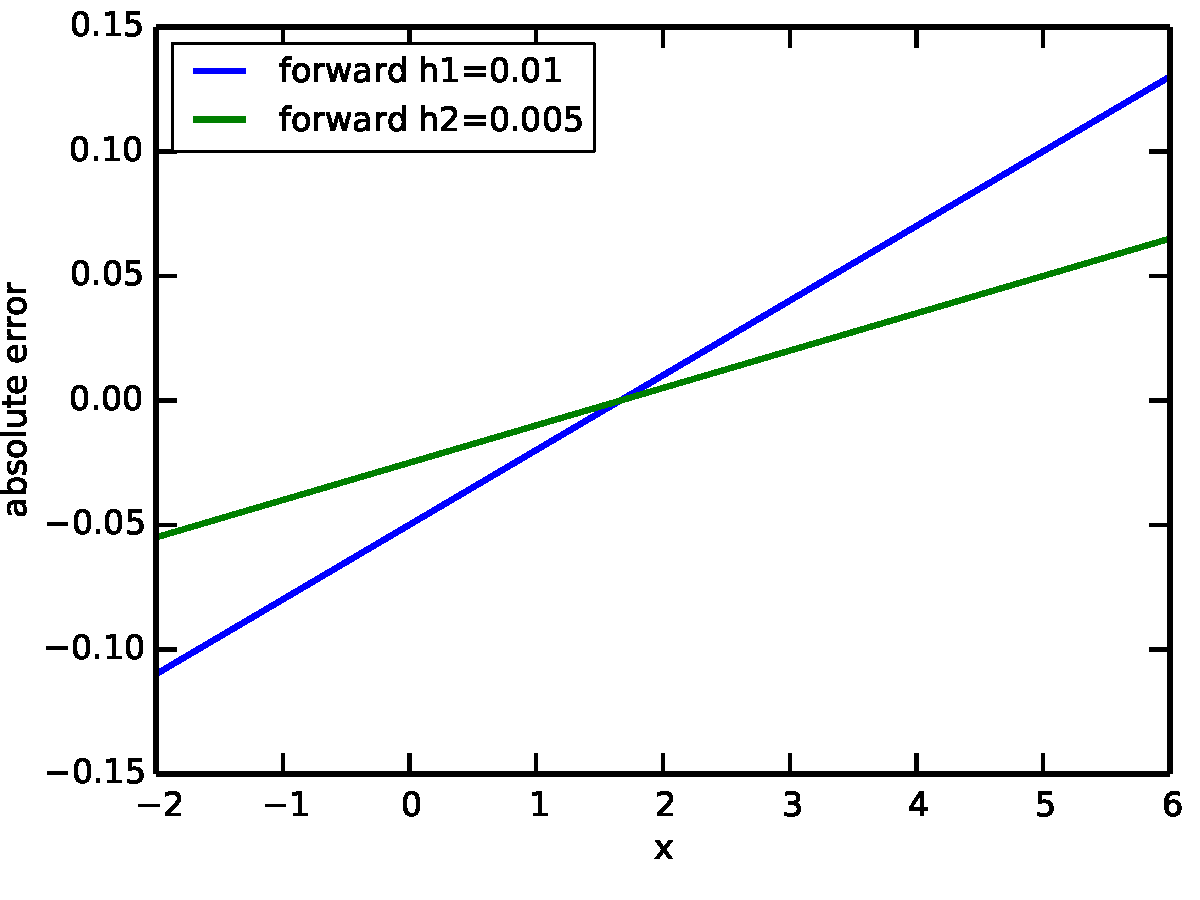
\includegraphics[width={0.49\textwidth}]{fig1.pdf} &
    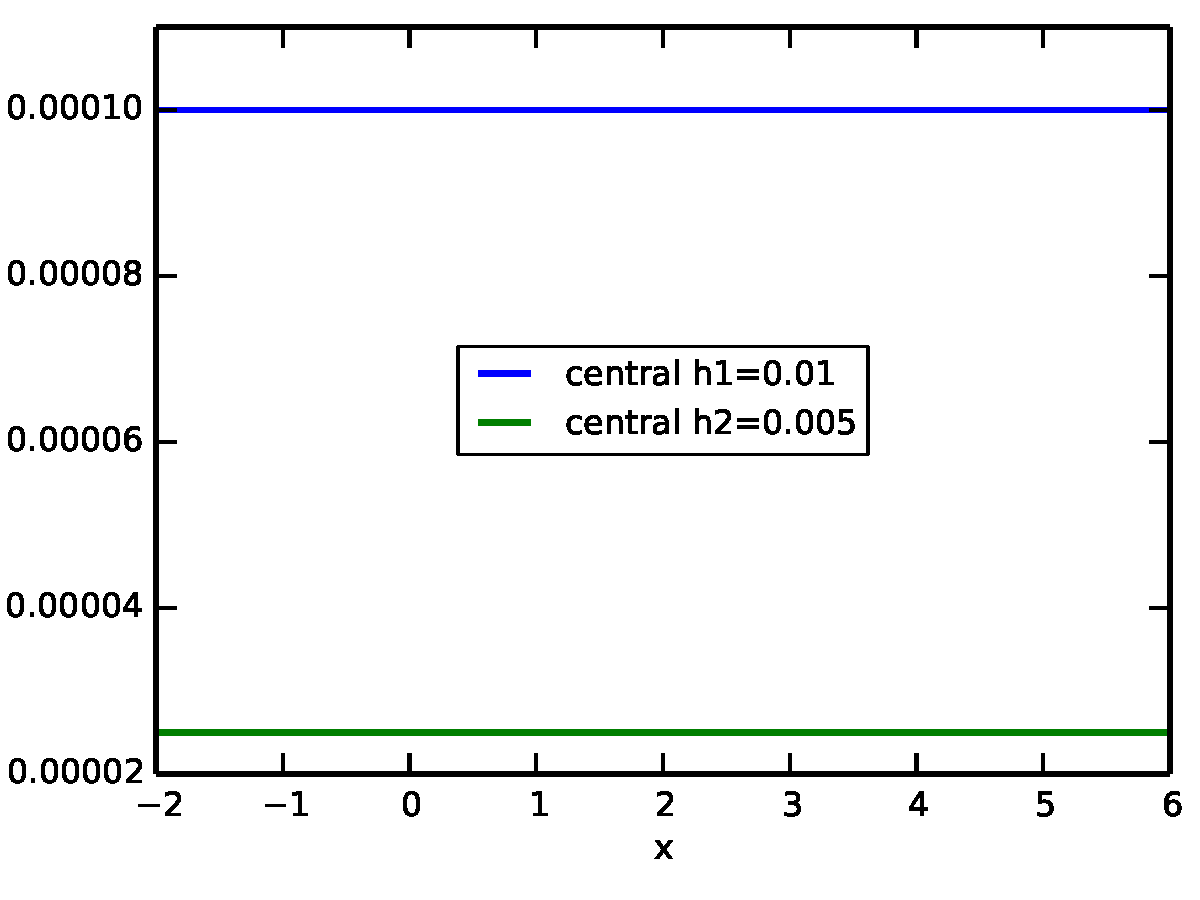
\includegraphics[width={0.49\textwidth}]{fig2.pdf} \\
\end{tabular}
\caption{Finite Difference}
\label{fig1}
\end{figure}


\section{Second Derivative}
Given that
\begin{equation}
  f(x_0+h) = f(x_0) + f'(x_0)~h + \frac{1}{2!} f''(x_0)~h^2 + \frac{1}{3!} f'''(x_0)~h^3 + O(h^4)
\end{equation}
and that
\begin{equation}
  f(x_0-h) = f(x_0) - f'(x_0)~h + \frac{1}{2!} f''(x_0)~h^2 - \frac{1}{3!} f'''(x_0)~h^3 + O(h^4) ,
\end{equation}
summing over these two equations, we have 
\begin{equation}
  f''(x_0) = \frac{f(x_0+h) + f(x_0-h) -2~f(x_0)}{h^2} + O(h^2) .
\end{equation}
This is an epression for second derivative at $x_0$ to the second order.


\section{Interpolation: Cepheid Lightcurve}
For this problem, I do not intend to bother myself writing the code on my own. Instead, I would rather use scipy library routines, as I guess the philosophy of this question is to observe the difference between different interpolation methods. 

For Lagrange polynomial interpolation, there is a python routine {\tt scipy.interpolate.lagrange}. As piecewise linear and quadratic interpolation, I use the routine {\tt scipy.interpolate.interp1d}, with keyword {\tt kind}=`{\tt linear}' and `{\tt quadratic}', respectively. I plot the results in Figure~\ref{fig2} and I zoom in the plot on the right panel in order to show the difference of other methods beside Lagrange interpolation. 

\begin{figure}
\centering
\begin{tabular}{cc}
    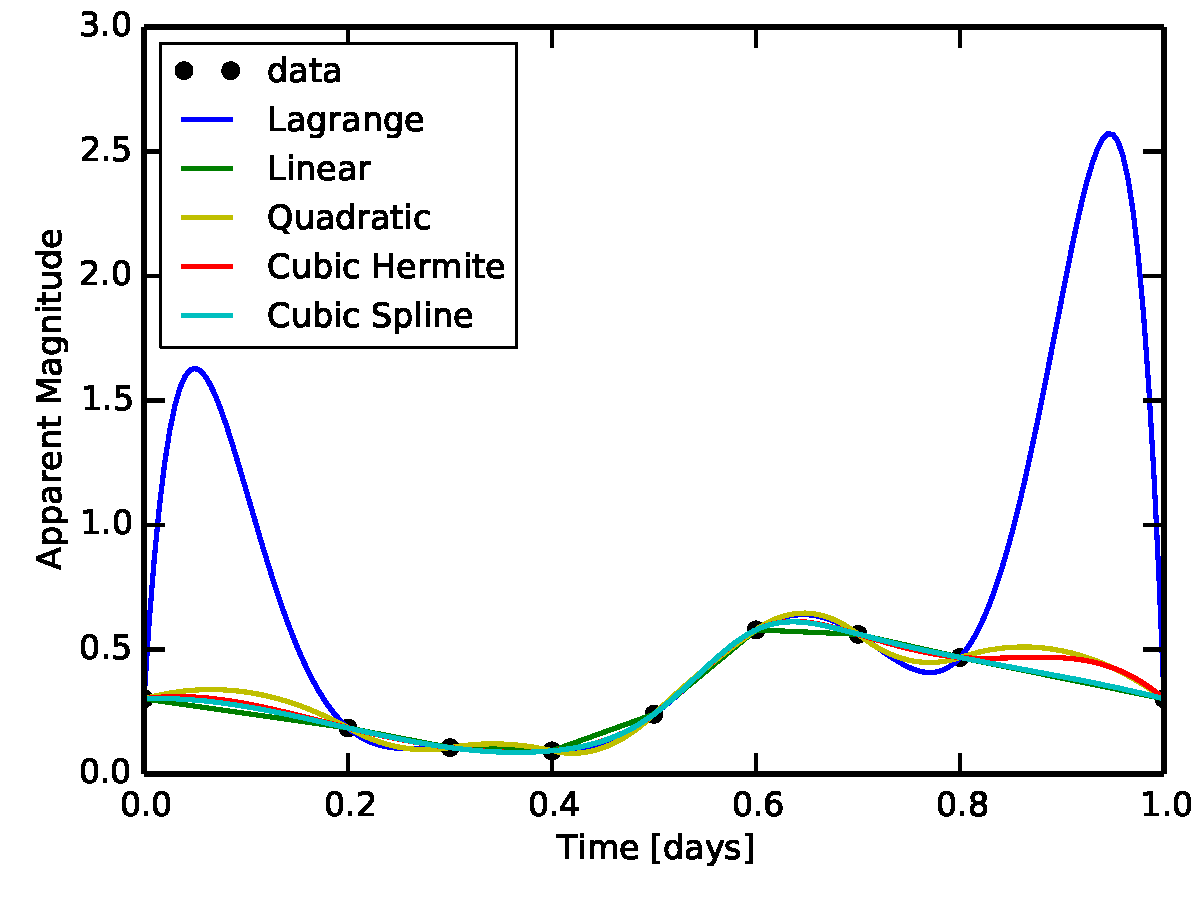
\includegraphics[width={0.49\textwidth}]{fig3.pdf} &
    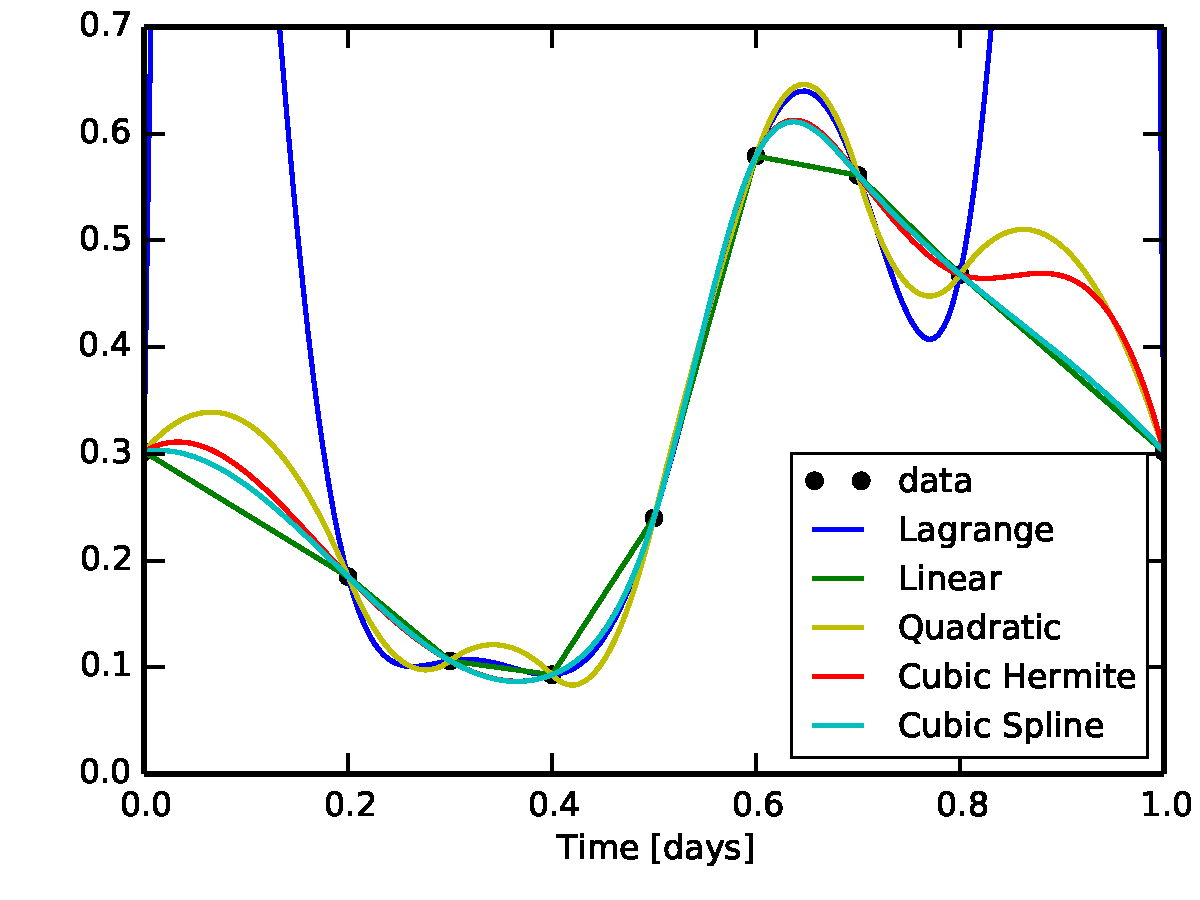
\includegraphics[width={0.49\textwidth}]{fig4.pdf} \\
\end{tabular}
\caption{Different Interpolation}
\label{fig2}
\end{figure}

\section{More Cepheid Lightcurve Interpolation}
Regarding cubic Hermite interpolation, I will insist use python routine {\tt scipy.interpolate.interp1d}, with keyword {\tt kind}=`{\tt cubic}'. For the natural cubic spline interpolation, there are two python routines {\tt scipy.interpolate.splrep} and {\tt scipy.interpolate.splev} combined can do this job, with keyword $k=3$ for a cubic spline. I plot the result in Figure~\ref{fig2} as well as a comparison.


\small
\section*{Appendix}
For a full description of the files here, find the ``README" file. \\
My team partner is Daniel Kong.

\end{document}
